\chapter{Background and System Architecture}
\label{chap:background}


The Keystone framework is built on the RISC-V instruction set architecture, which provides a unique foundation for secure system design due to its open specification and modular extensibility. Unlike traditional ISAs that are controlled by single vendors, RISC-V encourages community-driven enhancements and supports custom extensions, making it particularly attractive for trusted computing research and development. Its clean and well-documented privilege model allows for the implementation of isolation mechanisms that are critical to the construction of TEEs.

RISC-V defines three primary privilege levels: user mode (U-mode), supervisor mode (S-mode), and machine mode (M-mode). These privilege levels are hierarchical, with M-mode having the highest authority over system resources. M-mode has direct access to all hardware features and is responsible for critical functions such as interrupt control, exception handling, and access to physical memory protection mechanisms. Keystone leverages this privilege model by placing its Security Monitor (SM)—the core of the TCB—in M-mode. The SM is responsible for managing enclaves, enforcing memory isolation, and mediating access to sensitive system operations. By situating the TCB in M-mode, Keystone ensures that enclave isolation policies are enforced at the highest level of privilege, thereby minimizing the attack surface.

A central hardware feature used by Keystone is Physical Memory Protection (PMP), introduced in version 1.10 of the RISC-V Privilege Specification. PMP enables M-mode software to define access permissions for specific physical memory regions, controlling which lower-privilege modes (U and S) may read, write, or execute code in those regions. This capability forms the basis of Keystone’s memory isolation model. Each enclave is allocated a private memory region protected by PMP, ensuring that neither the host operating system nor any unauthorized software can access its contents. PMP rules are enforced directly by hardware, providing strong guarantees of isolation that are resistant to software-based attacks.

In addition to memory protection, RISC-V supports a flexible trap and exception handling mechanism. M-mode can intercept and handle all traps, but may delegate certain classes of exceptions—such as system calls and page faults—to S-mode for performance optimization. This delegation allows the enclave runtime to cooperate with the host operating system for memory management tasks, while still maintaining strict control over enclave boundaries. The virtual memory subsystem is managed through the standard RISC-V MMU, which translates virtual addresses to physical addresses using multi-level page tables. Keystone leverages this infrastructure to support enclaves that operate with their own private address spaces, protected by PMP from tampering or inspection.

Importantly, the use of standard programming models and toolchains for M-mode software development makes the Keystone Security Monitor both maintainable and extensible. Unlike microcode or hardwired logic, which are difficult to audit and update, the SM is implemented in C and can be subjected to conventional testing and formal verification techniques. This increases the transparency and trustworthiness of the TCB, which is a critical requirement for secure system design.

Taken together, the combination of RISC-V’s privilege hierarchy, PMP, trap delegation mechanisms, and extensibility provides a solid foundation for implementing robust and configurable TEEs. The Keystone framework capitalizes on these features to deliver a flexible and open platform for secure enclave execution, while remaining faithful to the RISC-V philosophy of openness and modularity.

\section{Trusted Execution Environments}
Trusted Execution Environments (TEEs) represent a class of hardware-assisted secure computing technologies that provide strong guarantees for the confidentiality and integrity of both code and data, even in systems where the underlying operating system or application software may be compromised. TEEs are designed to protect sensitive computations from a wide range of adversaries by establishing isolated execution contexts—commonly referred to as enclaves—through a combination of hardware features and privileged system software.

A TEE isolates a subset of the system’s resources, including CPU registers, memory, and I/O peripherals, and makes them accessible only to trusted applications executing within the enclave boundary. This isolation is enforced by the processor’s privilege mechanisms, memory protection units, or dedicated security monitors, ensuring that unauthorized entities—whether kernel-level malware or user-space processes—cannot access or tamper with enclave-resident assets.

Security within a TEE is achieved by reducing the size and complexity of the Trusted Computing Base (TCB). The TCB encompasses the set of components that must be trusted for the TEE to function securely. A minimal TCB is desirable, as it reduces the likelihood of vulnerabilities and simplifies formal verification and auditing processes. Modern TEEs aim to move as few components as possible into the TCB, while still providing robust isolation and essential services.

Prominent commercial TEE implementations include Intel Software Guard Extensions (SGX) and ARM TrustZone. Intel SGX facilitates the creation of enclaves at the user level, with memory encryption and access control enforced by hardware. ARM TrustZone, in contrast, provides a split-world architecture that partitions the processor into a secure world and a normal world, with secure world execution isolated via monitor calls. While these solutions have been successfully deployed in many real-world systems, their proprietary nature, rigid designs, and opaque implementations inhibit their utility for research, experimentation, and system-level innovation.

In response to these limitations, open-source TEE frameworks such as Keystone have emerged. Keystone is built atop the RISC-V instruction set architecture (ISA), which is itself open, extensible, and amenable to security-centric innovation. RISC-V’s modularity enables the design of TEEs that are both highly customizable and more transparent in their operation. A foundational architectural principle shared by all TEEs, including Keystone, is privilege separation. This concept involves executing the core TCB in a highly privileged execution mode—such as machine mode (M-mode) in RISC-V—while relegating the operating system and general-purpose applications to less privileged levels. This separation is crucial for enforcing isolation policies and preventing untrusted software from influencing the secure execution environment.

By leveraging privilege separation, physical memory protection, and modular TCB design, TEEs provide a powerful framework for secure computation in adversarial environments. Keystone builds upon these principles and extends them with openness and configurability, making it a valuable platform for academic and practical exploration of TEE technologies.

\section{Keystone architecture overview}

Keystone is an open-source Trusted Execution Environment (TEE) framework designed specifically for the RISC-V architecture. It enables the development of secure enclaves that are customizable, lightweight, and suitable for both research and deployment in resource-constrained or security-critical environments. Keystone’s design reflects a modular approach, emphasizing minimalism in its Trusted Computing Base (TCB), portability across RISC-V platforms, and extensibility to accommodate advanced security features. \cite{Lee2019}

The Keystone architecture operates across the multiple privilege levels defined by the RISC-V specification: user mode (U-mode), supervisor mode (S-mode), and machine mode (M-mode). These privilege levels are central to the enforcement of security policies within the system. Keystone's Security Monitor (SM), the heart of its TCB, executes in M-mode and holds exclusive authority over enclave lifecycle management, memory protection configuration, and enforcement of access control policies.

A typical Keystone-enabled platform consists of RISC-V processor cores augmented with secure boot mechanisms, trusted entropy sources, and optional hardware accelerators for cryptographic operations or secure I/O. Keystone does not mandate specific hardware features beyond RISC-V compliance and PMP (Physical Memory Protection), thereby supporting a broad spectrum of implementations from FPGA prototypes to silicon SoCs.

The SM, implemented in C and compiled as a standalone binary, embodies the critical logic responsible for managing the creation, execution, and destruction of enclaves. During enclave creation, the SM validates the enclave's memory layout, initializes its metadata, and configures PMP to ensure that only the SM and the enclave itself can access the designated memory regions. Once enclave execution begins, transitions between host and enclave contexts are mediated by the SM, which dynamically adjusts PMP settings to preserve strict isolation.

Each enclave is composed of two software layers: a user-level application (eapp) and a supervisor-level runtime environment. The eapp contains application-specific logic, while the runtime provides essential operating system abstractions such as exception handling, system call support, and virtual memory management. This two-tiered design allows for flexible enclave development and reduces the complexity of the eapp, which remains entirely untrusted by the host operating system.

The enclave lifecycle encompasses three primary stages: creation, execution, and destruction. During creation, the untrusted host allocates a contiguous region of physical memory—known as Enclave Page Memory (EPM)—to hold the enclave’s code, data, and page tables. This memory is populated and locked by the SM using PMP. In the execution phase, the SM facilitates entry into and exit from the enclave, ensuring that context switches maintain enclave confidentiality. Finally, destruction involves securely erasing enclave memory and releasing resources to prevent post-mortem data leakage.

Keystone also supports optional features such as remote attestation, allowing third-party verifiers to authenticate enclave state before provisioning sensitive data. Additionally, the architecture can be extended to support secure I/O pathways, cryptographic acceleration, and debugging features useful for both development and runtime monitoring.

\begin{figure}[htbp]
\centering
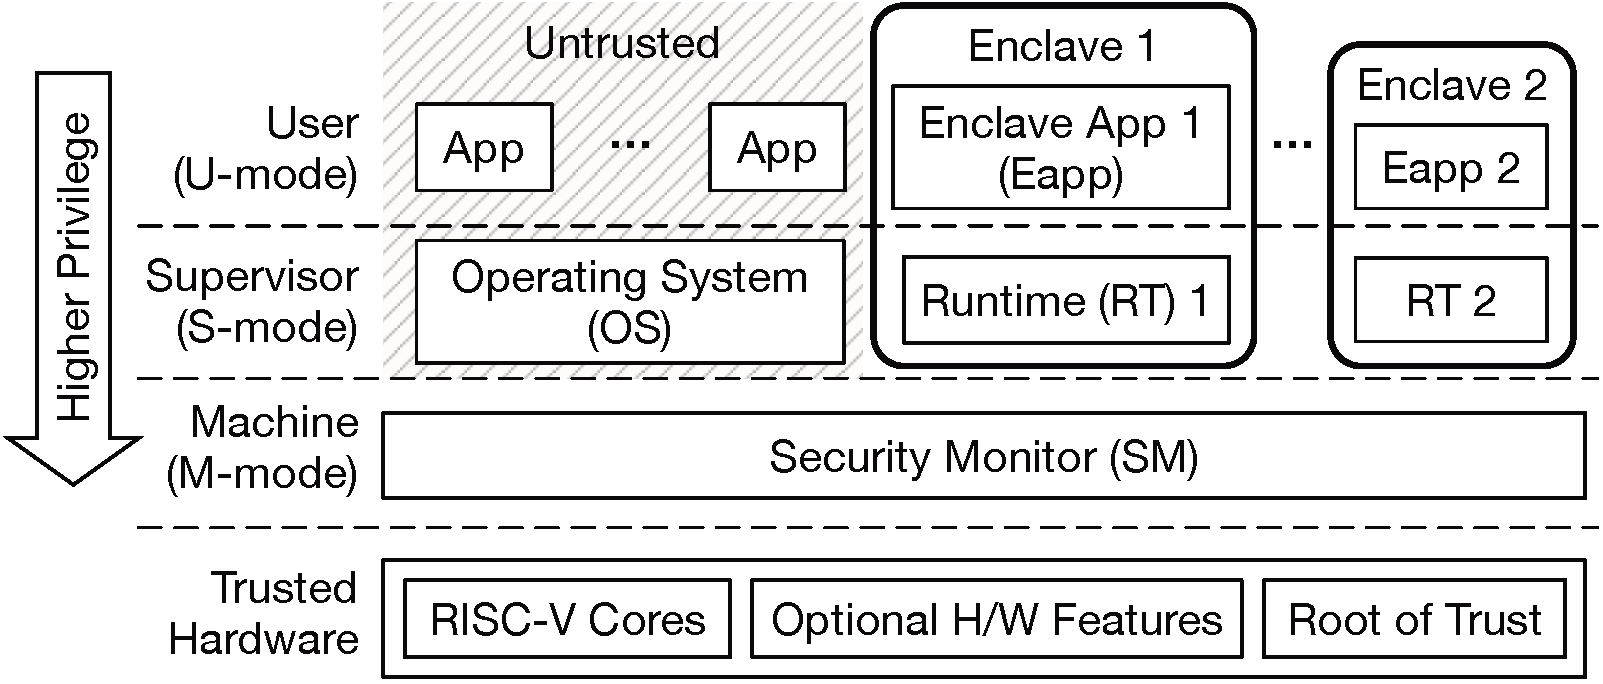
\includegraphics[width=0.9\linewidth]{figures/keystone_overview.png}
\caption{Overview of the Keystone architecture illustrating components such as the Security Monitor, enclave runtime, and the privilege hierarchy.}
\label{fig:keystone_overview}
\end{figure}

\begin{figure}[htbp]
\centering
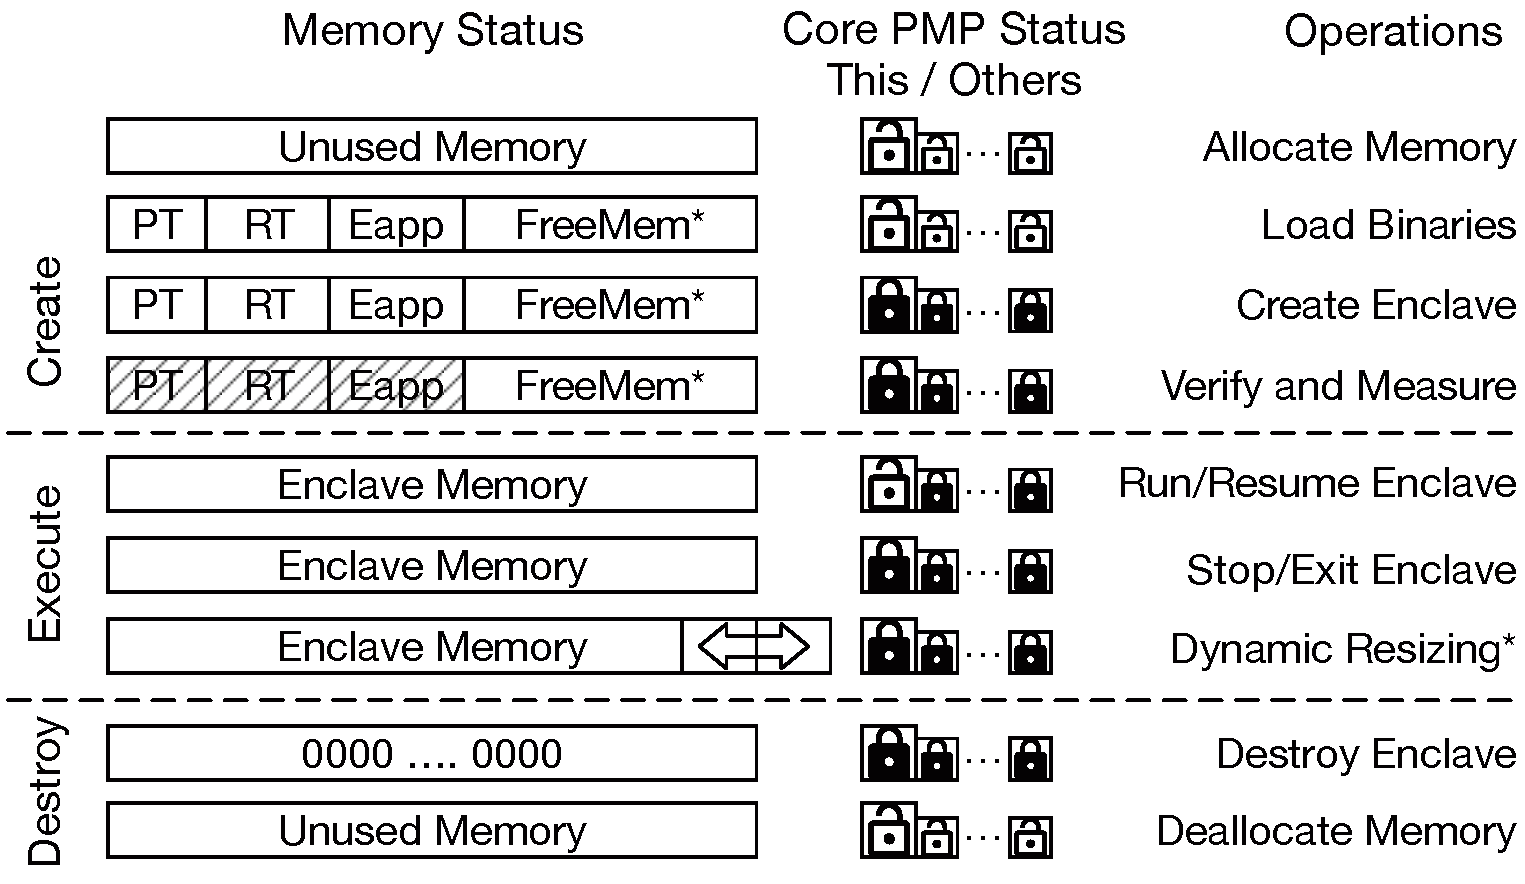
\includegraphics[width=0.9\linewidth]{figures/enclave_lifecycle.png}
\caption{Stages of a Keystone enclave lifecycle: creation, execution, and destruction.}
\label{fig:enclave_lifecycle}
\end{figure}

Overall, Keystone provides a clean, modular, and research-oriented TEE framework that leverages the openness of RISC-V to deliver both strong security guarantees and development flexibility. Its layered architecture, minimal TCB, and standards-compliant interfaces make it a compelling platform for building and evaluating secure applications on next-generation processors.

\section{Comparison with other TEEs}

Keystone distinguishes itself from existing commercial Trusted Execution Environment (TEE) implementations, such as Intel Software Guard Extensions (SGX) and ARM TrustZone, through its open-source nature, customizable architecture, and alignment with the RISC-V ecosystem. While SGX and TrustZone have been widely deployed in commodity hardware and offer robust isolation features, they are constrained by their proprietary designs, large and opaque TCBs, and limited extensibility, which make them less suitable for academic research and fine-grained system-level customization.

ARM TrustZone utilizes a dual-world execution model, dividing the processor into a Secure World and a Normal World. The system transitions between these worlds using secure monitor calls (SMCs). Each world operates with its own set of execution contexts and memory spaces. In the Secure World, a trusted operating system—such as OP-TEE—executes sensitive applications that conform to the GlobalPlatform TEE Internal API. However, TrustZone’s architecture supports only a single secure world instance, lacks support for dynamic enclave creation, and requires significant overhead for world switches, especially in the handling of interrupts. Moreover, the TCB in TrustZone is relatively large, encompassing the entire Secure World kernel and trusted services, which complicates formal verification and increases the risk of vulnerabilities.

Intel SGX, in contrast, supports dynamic creation of enclaves at runtime within the address space of user-space processes. These enclaves are protected by a memory encryption engine and execute in ring 3, isolated from both the operating system and hypervisor. Communication between host and enclave is facilitated by ECALL and OCALL mechanisms, whose interfaces are defined through the edger8r tool. While SGX offers strong isolation and cryptographic sealing of enclave contents, it imposes rigid constraints on enclave memory size and structure. Notably, SGX enclaves do not support supervisor-level execution, limiting the complexity of software that can be securely encapsulated within the enclave. Additionally, SGX is tightly bound to Intel hardware, restricting portability and experimentation.

Keystone integrates the strengths of both TrustZone and SGX while addressing their limitations through an open and modular framework. Its architecture supports dynamic enclave creation, hierarchical privilege separation (via user and supervisor modes), and execution control via a minimal M-mode Security Monitor. Enclave memory is isolated using RISC-V’s Physical Memory Protection (PMP) features, which are dynamically configured by the SM to enforce strict access control. This enables strong spatial and temporal memory isolation without relying on hardware-bound limitations or encryption mechanisms.

Keystone also supports a lightweight communication interface, dubbed keyedger, which serves a similar role to edger8r in SGX, but is designed to be more flexible and extensible. While it currently offers partial support for the GlobalPlatform TEE Internal API, Keystone’s modularity allows it to be extended to support custom APIs and protocols suited to specific use cases or research goals.



Through its combination of openness, modularity, and hardware-agnostic design, Keystone offers a uniquely research-friendly and extensible platform for investigating and deploying secure enclaves. It enables hardware/software co-design, supports verifiable security primitives, and aligns with emerging open hardware ecosystems, positioning it as a forward-looking alternative to incumbent TEE technologies.

\section{Performance considerations in TEEs}